\documentclass[twoside]{article}
\usepackage[T1]{fontenc}
\usepackage{geometry}
\geometry{verbose}
\usepackage{fancyhdr}
\pagestyle{fancy}
\setlength\parskip{\medskipamount}
\setlength\parindent{0pt}
\usepackage{graphicx}
\usepackage{fmtcount}
\usepackage{enumerate}
\usepackage{mathrsfs}

% for printing from gpgl
%\topmargin=-0.25in
%\voffset=-10pt
%\textwidth=7.0in
% values for gpg5 and Ricoh printer.
\topmargin=0.75in
\headheight=0.125in
\headsep=0.25in
\topskip=0pt
\voffset=-30pt
\textwidth=6.5in
% common values
\oddsidemargin=0in
\evensidemargin=0in
\textheight=9.0in

% introduce new commands here.
\makeatletter % changes the catcode of @ to 11

% two new commands to do labelling. - gpg 12/4/13
\newcommand{\customlabel}[2]{%
\protected@write \@auxout {}{\string \newlabel {#1}{{#2}{}}}}

\newcommand{\actlabel}[1]{%
\protected@write \@auxout {}{\string \newlabel {#1}{{\arabic{activity}}{}}}}

%% Special footnote code from the package 'stblftnt.sty' needed to put footnote
%% on section title
%% Author: Robin Fairbairns -- Last revised Dec 13 1996
\let\SF@@footnote\footnote
\def\footnote{\ifx\protect\@typeset@protect
    \expandafter\SF@@footnote
  \else
    \expandafter\SF@gobble@opt
  \fi
}
\expandafter\def\csname SF@gobble@opt \endcsname{\@ifnextchar[%]
  \SF@gobble@twobracket
  \@gobble
}
\edef\SF@gobble@opt{\noexpand\protect
  \expandafter\noexpand\csname SF@gobble@opt \endcsname}
\def\SF@gobble@twobracket[#1]#2{}

\makeatother % changes the catcode of @ back to 12
% end of new commands.

\newcounter{activity}

\begin{document}


\title{Investigative Physics\\ Activity Units for IQS Physics-S1}


\author{E.F. Bunn,$^1$ M.S. Fetea,$^1$
G.P. Gilfoyle,$^1$ H. Nebel,$^1$ S.Serej,$^1$ \\ P.D. Rubin,$^2$ and M.F. Vineyard$^3$\\[8pt]
$^1$Department of Physics, University of Richmond, VA 23173 \\[4pt]
$^2$Department of Physics, George Mason University, Fairfax, VA  22030 \\[4pt]
$^3$Department of Physics, Union College, Schenectady, NY 12308}

\maketitle
\begin{abstract}
The exercises in this manual have been developed to support an investigative
physics course that emphasizes active learning. Some of these units have been
taken from the Workshop Physics project at Dickinson College and the Tools for
Scientific Thinking project at Tufts University and modified for use at the
University of Richmond. Others have been developed locally.

The units are made up of activities designed to guide your investigations in
the laboratory. The written work will consist primarily of documenting your
class activities by filling in the entries in the spaces provided in the units.
The entries consist of observations, derivations, calculations, and answers
to questions. Although you may use the same data and graphs as your partner(s)
and discuss concepts with your classmates, all entries should reflect your own
understanding of the concepts and the meaning of the data and graphs you are
presenting. Thus, each entry should be written in your own words. Indeed, it
is very important to your success in this course that your entries reflect a
sound understanding of the phenomena you are observing and analyzing.

We wish to acknowledge the support we have received for this project from the
University of Richmond and the Instrumentation and Laboratory Improvement program 
of the National Science Foundation. Also, we would like to thank our laboratory 
directors for their invaluable technical assistance.
\end{abstract}


\begin{center}

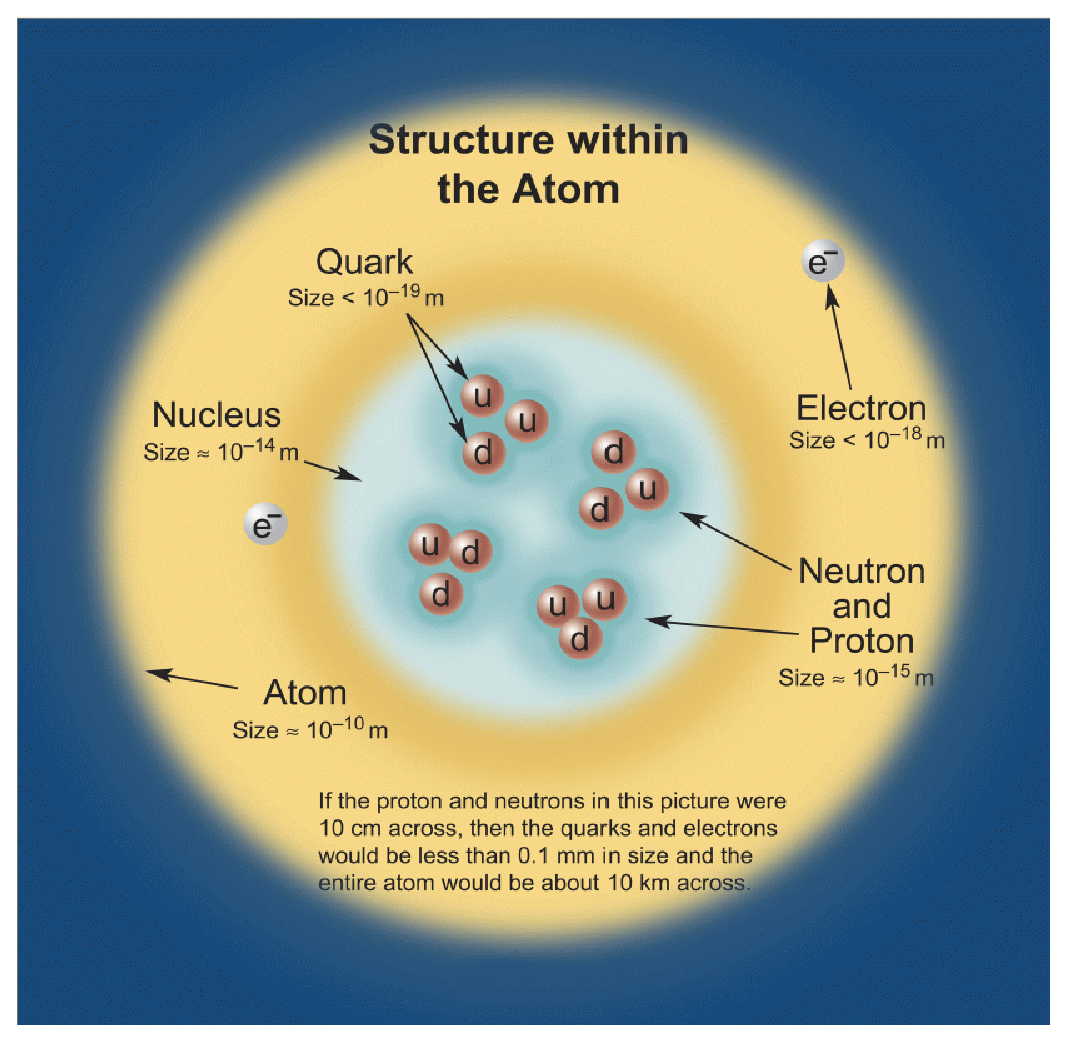
\includegraphics[width=3.4in]{AtomicStructure.ps}

\end{center}

\thispagestyle{empty}

\newpage


\ 
\setcounter{page}{1}

\vfill

Cover art: The atom consists of smaller electrons and a nucleus consisting of protons and neutrons.
The protons and neutrons, in turn, are formed from objects called quarks and gluons.
Courtesy, the American Institute of Physics.

\pagebreak

\tableofcontents{}

\newpage

\setcounter{page}{3}

\thispagestyle{plain}

\vfill

\ 

\pagebreak

\setcounter{activity}{0}
\section{Work and Kinetic Energy\footnote{1990-93 Dept. of Physics and Astronomy, Dickinson College. Supported by FIPSE
(U.S. Dept. of Ed.) and NSF. Portions of this material have been modified locally
and may not have been classroom tested at Dickinson College.}}

Name \rule{2.0in}{0.1pt}\hfill{}Section \rule{1.0in}{0.1pt}\hfill{}Date \rule{1.0in}{0.1pt}

\textbf{Objectives }

\begin{itemize}
\item To extend the intuitive notion of work as physical effort to a formal mathematical
definition of work as a function of force and distance. 
\item To discover Hooke's law. 
\item To understand the concept of kinetic energy and its relationship to work as
embodied in the work-energy theorem.
\end{itemize}

\textbf{Apparatus }

\begin{center}
\begin{tabular}{lll}
spring scale            & variety of masses & support rod to hand spring\\
wooden block with hook  & large spring      & 2-meter stick \\
\end{tabular}
\end{center}

\textbf{The Concept of Physical Work }

Suppose you are president of the Richmond Load 'n' Go Co. A local college has
three jobs available and will allow you to choose which one you want before
offering the other two jobs to rival companies. All three jobs pay the same
amount of money. Which one would you choose for your crew? 
\textbf{NOTE:} The quantities in this figure are given in British units, 
where ``pounds'' = $mg$, not just $m$, i.e. the $g$ is already included.

\vspace{0.3cm}
{\par\centering 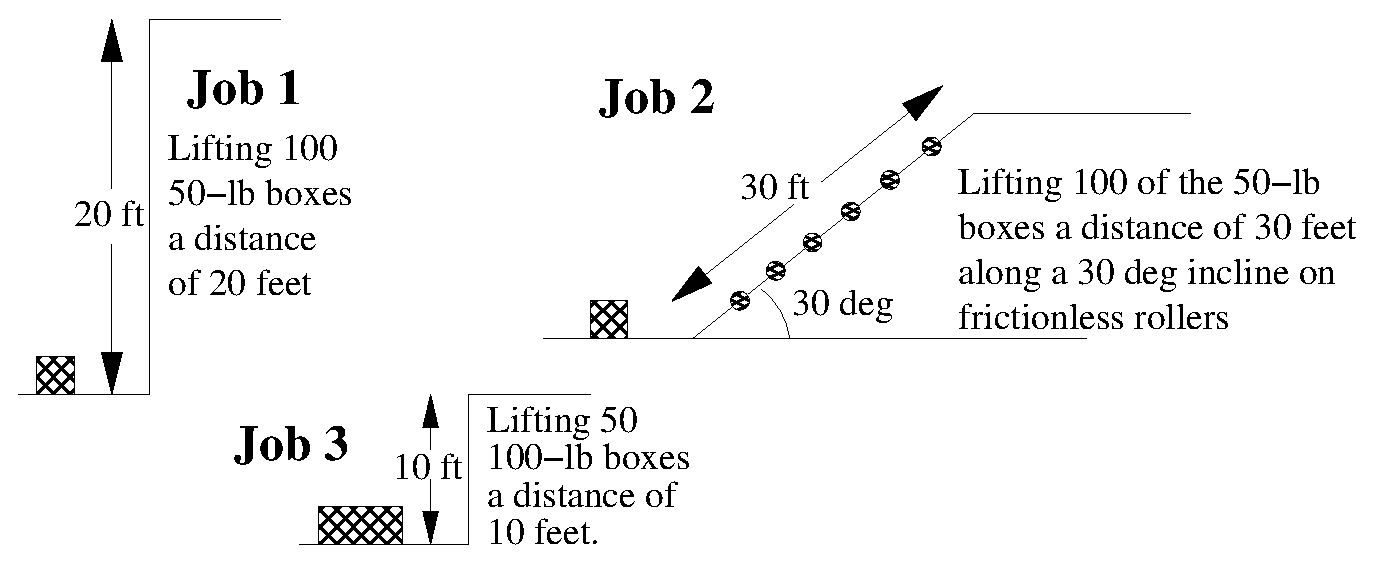
\includegraphics[width=5.5in]{workAndKE/work_power_fig1b.eps} \par}
\vspace{0.3cm}

\textbf{Activity  \stepcounter{activity}\arabic{activity}: Choosing Your Job }

Examine the descriptions of the jobs shown in figure above. Which one would
you be most likely to choose? Least likely to choose? Explain the reasons for
your answer.
\vspace{30mm}

You obviously want to do the least amount of work for the most money. Before
you reconsider your answers later in this unit, you should do a series of activities
to get a better feel for what physicists mean by work and how the president
of Load 'n' Go can make top dollar.

\vspace{0.3cm}
{\par\centering 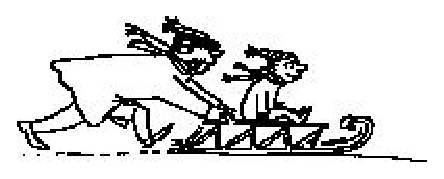
\includegraphics{workAndKE/work_power_fig2.eps} \par}
\vspace{0.3cm}

In everyday language we refer to doing work whenever we expend effort. In order
to get an intuitive feel for how we might define work mathematically, you should
experiment with moving your textbook back and forth along a table top and a
rougher surface such as a carpeted floor.

\textbf{Activity  \stepcounter{activity}\arabic{activity}: This is Work!} 

(a) Pick a distance of a meter or so. Sense how much effort it takes to push
a heavy book that distance. How much more effort does it take to push it twice
as far? 
\vspace{20mm}

(b) Pile another similar book on top of the original one and sense how much
effort it takes to push the two books through the distance you picked. Comment
below.
\vspace{20mm}

(c) If the ``effort'' it takes to move an object is associated
with physical work, guess an equation that can be used to define work mathematically
when the force on an object and its displacement (i.e., the distance it moves)
lie along the same line.
\vspace{20mm}

In physics, work is not simply effort. In fact, the physicist's definition of
work is precise and mathematical. In order to have a full understanding of how
work is defined in physics, we need to consider its definition in a very simple
situation and then enrich it later to include more realistic situations.

\textbf{A Simple Definition of Physical Work:} If an object that is moving in
a straight line experiences a constant force in the direction of its motion
during the time it is undergoing a displacement, the work done by the external
force, \( F_{ext} \), is defined as the product of the force and the displacement of the object, 
\[
W=F_{ext}\Delta x\]


where $W$ represents the work done by the external force, \( F_{ext} \) is the
magnitude of the force, and \( \Delta  x\) is the displacement of the object.
%WHY THE HECK DO WE SAY THIS:
%{\bf I WANT TO DROP THIS SENTENCE:} Work done by a force is always positive!

What if the force of interest and the displacement are in opposite directions? For instance, what about the work done by the force of sliding friction,
\( F_{f} \), when a block slides on a rough surface? The work done by the friction force is
\[
W_{f}=-F_{f}\Delta x\]
%YUCK:
%{\bf AND THIS ONE:} Work done against a force is always negative!

\newpage

\textbf{Activity  \stepcounter{activity}\arabic{activity}: Applying the Physics Definition of Work} 

(a) Does effort necessarily result in physical work? Suppose two guys are in
an evenly matched tug of war. They are obviously expending effort to pull on the
rope, but according to the definition of physical work, are they doing any physical
work? Explain.

\vspace{0.3cm}
{\par\centering 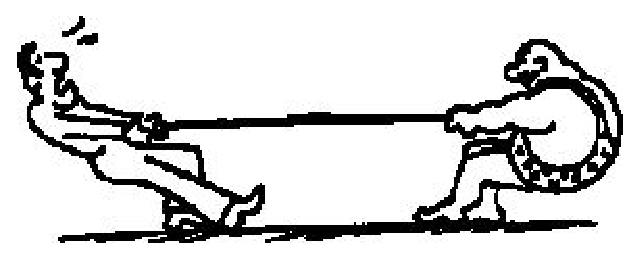
\includegraphics{workAndKE/work_power_fig3.eps} \par}
\vspace{0.3cm}

(b) A wooden block with a mass of 0.30 kg is pushed along a sheet of ice that
has no friction with a constant external force of 10 N which acts in a horizontal
direction. After it moves a distance of 0.40 m how much work has been done on
the block by the external force?
\vspace{20mm}

(c) The same wooden block with a mass of 0.30 kg is pushed along a table with
a constant external force of 10 N which acts in a horizontal direction. It moves
a distance of 0.40 m. However, there is a friction force opposing its motion with magnitude 
$|{\bf F}_{friction}| = \mu N$ where $N$ is the normal force exerted on the block by by the table.
Here $N$ is perpendicular to the surface of the table and equal to the weight of the block (since the table
is holding up the block).
The coefficient of sliding friction $\mu$ is an experimental factor that relates $N$ to the friction force.
Here \( \mu _{k} \), is 0.20. 

\vspace{0.3cm}
{\par\centering 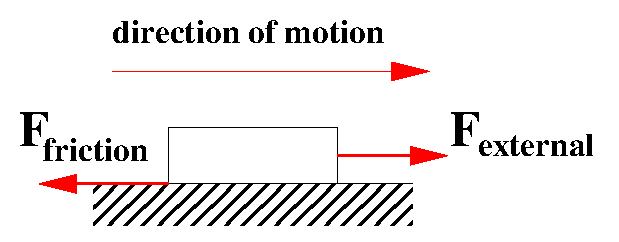
\includegraphics[height=1in]{workAndKE/work_power_fig4b.eps} \par}
\vspace{0.3cm}

\begin{enumerate}
\item According to the definition of work done by a force, what is the work associated with the external force? 
Is the work positive or negative? Show your calculation.\vspace{20mm}

\item According to our discussion above of the work done by a friction force, 
what is the work associated with the friction force? 
Is the work positive or negative? Show your calculation.\vspace{20mm}

\end{enumerate}

\newpage

(d) Suppose you lift a 0.3 kg object through a distance of 1.0 m at a constant velocity.

\vspace{0.3cm}
{\par\centering 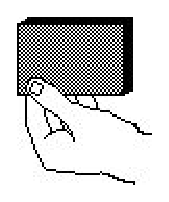
\includegraphics{workAndKE/work_power_fig5.eps} \par}
\vspace{0.3cm}

\begin{enumerate}
\item What is the work associated with the force that the earth exerts on the object? Is the work positive or negative? Show your calculation.
\vspace{20mm}

\item What is the work associated with the external force you apply to the object? Is the work positive or negative? Show your calculation.
\vspace{20mm}

\end{enumerate}
\textbf{Pulling at an Angle What Happens When the Force and the Displacement
Are Not Along the Same Line? }

Let's be more quantitative about measuring force and distance and calculating
the work. How should work be calculated when the external force and the displacement
of an object are not in the same direction?

\vspace{0.3cm}
{\par\centering 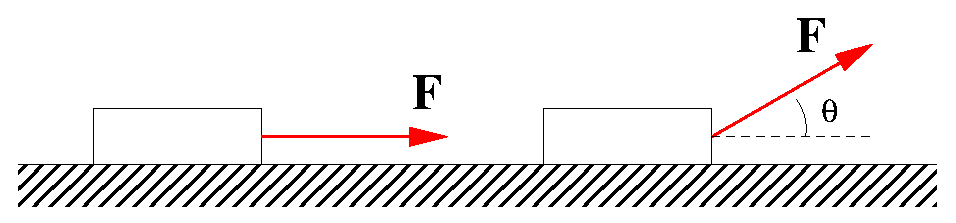
\includegraphics[width=5.5in]{workAndKE/work_power_fig6b.eps} \par}
\vspace{0.3cm}

To investigate this, you will use a spring scale to measure the force necessary
to slide a block along the table at a constant speed. Before you make your simple 
force measurements, you should put some weights on your block so that it slides 
along a smooth surface at a constant velocity even when it is being pulled with 
a force that is 30 or 60 degrees from the horizontal.

\textbf{Activity  \stepcounter{activity}\arabic{activity}: Calculating Work} 

(a) Hold a spring scale horizontal to the table and use it to pull the block
a distance of 0.5 meters along the horizontal surface in such a way that the
block moves at a constant speed. Record the force in newtons and the distance
in meters in the space below and calculate the work done on the block in joules.
(Note that there is a special unit for work, the joule, or J for short. 
One joule is equal to one newton times one meter, i.e., J = N\,m.)
\vspace{20mm}

\newpage

(b) Repeat the measurement, only this time pull on the block at a 30\( ^{\circ } \) 
angle with respect to the horizontal. 
Pull the block at about the same speed. Is the force needed larger or smaller than you measured in part (a)?
\vspace{20mm}

(c) Repeat the measurement once more, this time pulling the block at a 60\( ^{\circ } \) 
angle with respect to the horizontal.  
Pull the block at about the same speed as before.
\vspace{20mm}

(d) Assuming that the actual physical work done in part (b) is the same as the
physical work done in part (a) above, how could you enhance the mathematical
definition of work so that the forces measured in part (b) could be used to
calculate work? In other words, use your data to postulate a mathematical equation
that relates the physical work, $W$, to the magnitude of the applied force, $F$,
the magnitude of the displacement, \( \Delta  s\), and the angle, \( \theta  \),
between $F$ and \( \Delta  s\). Explain your reasoning. Hint: sin 30\( ^{\circ } \)
= 0.500, sin 60\( ^{\circ } \) = 0.866, cos 30\( ^{\circ } \) = 0.866, cos 60\( ^{\circ } \)
= 0.500.
\vspace{20mm}

\textbf{Work as a Dot Product }

Review the definition of dot (or scalar) product as a special product of two
vectors in your textbook, and convince yourself that the dot product can be
used to define physical work in general cases when the force is constant but
not necessarily in the direction of the displacement resulting from it. 
\[W={\bf F}\cdot {\bf \Delta s}\]


\textbf{Activity  \stepcounter{activity}\arabic{activity}: How Much Work Goes with Each Job? }

(a) Re-examine the descriptions of the jobs shown in the figure on the first
page of this experiment. What is the minimum physical work done in job 1? Note that the
 data are given in British units, so the work will be expressed in foot pounds (ft lbs), 
not newton meters. 
Remember, the ``pounds'' are $mg$, so you don't need to multiply by $g$.
\vspace{12mm}

(b) What is the minimum physical work done in job 2?
\vspace{12mm}

(c) What is the minimum physical work is done in job 3?
\vspace{12mm}

(d) Was your original intuition about which job to take correct? Which job should
Richmond Load 'n' Go try to land?
\vspace{12mm}

%----------------------------------------------------------------------------------------

\newpage

\textbf{The Force Exerted on a Mass by an Extended Spring} 

So far we have pushed and pulled on an object with a constant force and calculated
the work needed to displace that object. In most real situations the force on
an object can change as it moves. 

What happens to the average force needed to stretch a spring from 0 to 1 cm
compared to the average force needed to extend the same spring from 10 to 11
cm? How does the applied force on a spring affect the amount by which it stretches,
i.e., its displacement?

\textbf{Activity  \stepcounter{activity}\arabic{activity}: Are Spring Forces Constant?} 

Hang the spring from a support rod with the large diameter coils in the downward
position. Extend the spring from 0 to 1 cm. Feel the force needed to extend
the spring. Extend the spring from 10 to 11 cm. Feel the force needed to extend
the spring again. How do the two forces compare? Are they the same? 
\vspace{10mm}

\textbf{The Force and Work Needed to Stretch a Spring} 

Now we would like to be able to quantify the force and work needed to extend
a spring as a function of its displacement from an equilibrium position (i.e.,
when it is ``unstretched'').

\textbf{Activity  \stepcounter{activity}\arabic{activity}: Force vs. Displacement for a Spring }\actlabel{hooke}

(a) The table below shows the results of a series of measurements of the distance $s$ from the floor to
the position of a mass $m$ hung from a spring like the one you have.
Calculate and record the external force, \( F_{ext} \), 
and the stretch of the spring, \(x\) (\(= s_{0} - s\)), for each mass.
The last four columns will not be filled in until you get to Activities \ref{forceDistance} and \ref{work}.

\begin{center}
\begin{tabular}{|c|c|c|c|c|c|c|c|c|} \hline
$m$ (kg) & $s$ (m) & $ F_{ext} $ (N)  & $x$ (m) & $\Delta x$ (m) & $\langle x\rangle$ (m) & $\langle F_{ext}\rangle $ (N) & $\Delta W$ (J) & $ W_{total}$ (J) \\ \hline
0.0      &  1.508  &                 &         &                &                        &                               &                &                  \\ \hline
0.1      &  1.390  &                 &         &                &                        &                               &                &                  \\ \hline
0.2      &  1.220  &                 &         &                &                        &                               &                &                  \\ \hline
0.3      &  1.153  &                 &         &                &                        &                               &                &                  \\ \hline
0.4      &  1.032  &                 &         &                &                        &                               &                &                  \\ \hline
0.5      &  0.911  &                 &         &                &                        &                               &                &                  \\ \hline
0.6      &  0.789  &                 &         &                &                        &                               &                &                  \\ \hline
0.7      &  0.669  &                 &         &                &                        &                               &                &                  \\ \hline
0.8      &  0.547  &                 &         &                &                        &                               &                &                  \\ \hline
0.8      &  0.420  &                 &         &                &                        &                               &                &                  \\ \hline
1.0      &  0.301  &                 &         &                &                        &                               &                &                  \\ \hline
\end{tabular}
\end{center}

(b) Using \textit{Excel}, create a graph of \( F_{ext} \) (vertical axis) vs. $x$. 
Is the graph linear?
If the force, \( F_{ext} \), increases with the displacement in a proportional
way, fit the data to find the slope of the line. Insert a copy of the graph
into your notebook. Use the symbol $k$ to represent the slope of the line. What
is the value of $k$? What are its units? Note: 
$k$ is known as the spring constant.
\vspace{10mm}

(c) Write the equation describing the relationship between the external force,
\( F_{ext} \), and the total displacement, 
$x$, of the spring from its equilibrium
using the symbols \( F_{ext} \), $k$, and $x$.
\vspace{10mm}

Note: Any restoring force on an object which is proportional to its displacement
is known as a Hooke's Law Force. There was an erratic, contentious genius named
Robert Hooke who was born in 1635. He played with springs and argued with Newton.

\newpage

\textbf{Calculating Work when the Force is not Constant }

We would like to expand the definition of work so it can be used to calculate
the work associated with stretching a spring and the work associated with other
forces that are not constant. A helpful approach is to plot the average force
needed to move an object for each successive displacement \( \Delta  x\) as
a bar graph like that shown in the figure below. The figure shows a graph representing
the average applied force causing each unit of displacement of an object. This
graph represents force that is not constant but not the force vs. displacement
of a typical spring.

Note: The bar graph below is intended to illustrate mathematical concepts. Any
similarity between the values of the forces in the bar graph and any real set
of forces is purely coincidental. In general, the force causing work to be done
on an object is not constant.

\vspace{0.3cm}
%{\par\centering \includegraphics{work_kinetic_fig1.eps} \par}
{\par\centering 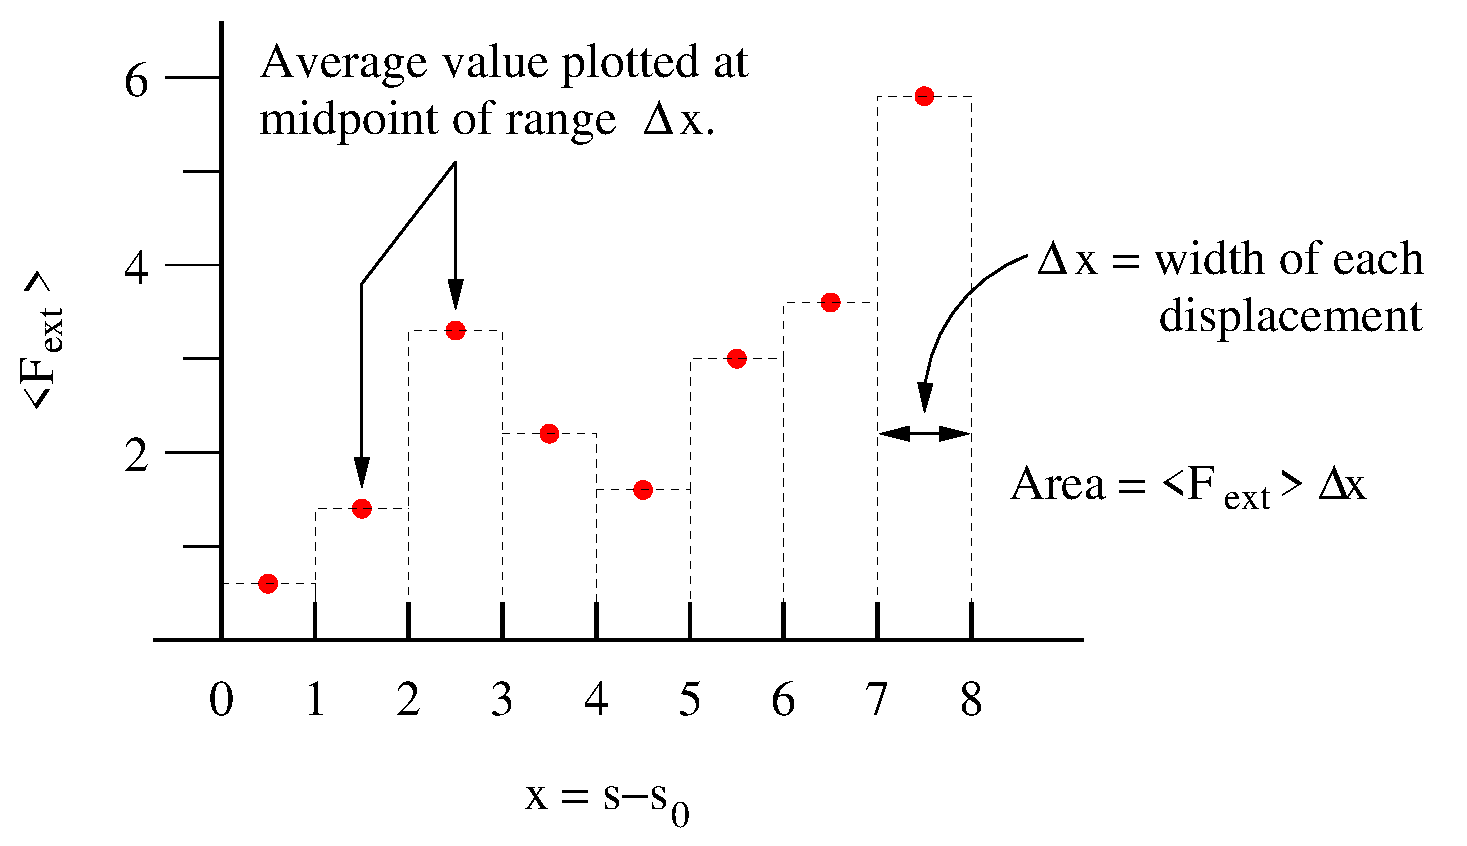
\includegraphics[width=6.0in]{workAndKE/workAndKEF1.eps} \par}
\vspace{0.3cm}

\textbf{Activity  \stepcounter{activity}\arabic{activity}: Force vs. Distance in a Bar Graph }\actlabel{forceDistance}

(a) Using your data from Activity \ref{hooke}, calculate the width of each displacement \( \Delta x \),
the average position for each displacement $\langle x \rangle$, 
and the average external force \(\langle F_{ext} \rangle\) for each displacement, 
and record the values in the table above. Plot \( \langle F_{ext} \rangle\) vs. $x$ 
as a bar graph on the grid below.  
(Choose appropriate scales for the axes before making the graph.)

\vspace{0.3cm}
%{\par\centering \includegraphics{work_kinetic_fig2.eps} \par}
{\par\centering 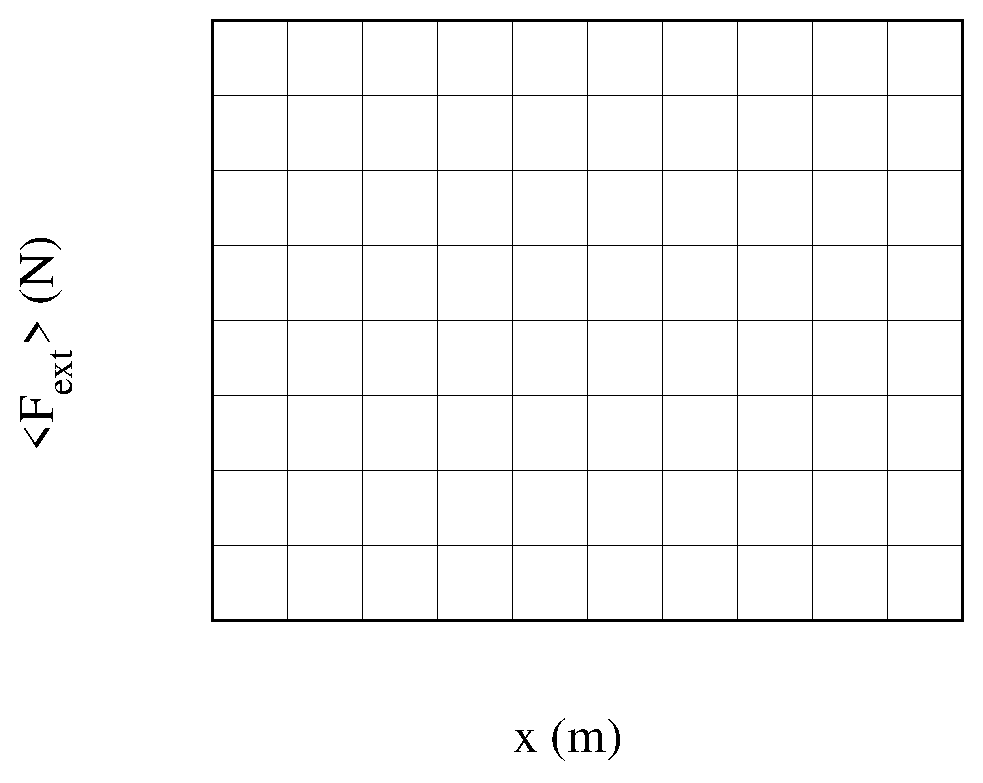
\includegraphics[width=6.0in]{workAndKE/workAndKEF2.eps} \par}
\vspace{0.3cm}

How can we calculate the work done in stretching the spring? We can use several
equivalent techniques: (1) adding up little pieces of \( \langle F_{ext} 
\rangle \Delta x \) from the above bar graph,
(2) finding the area under the ``curve'' you created in Activity \ref{hooke}, or (3)
using mathematical integration.

All three methods should yield about the same result. 
If you have studied integrals in calculus you may want to consult
your instructor or the textbook about how to set up the appropriate definite
integral to calculate the work needed to stretch the spring. 

\textbf{Activity  \stepcounter{activity}\arabic{activity}: Calculation of Work }\actlabel{work}

(a) Calculate the work needed to stretch the spring by adding up small increments of 
\( \langle F_{ext} \rangle \Delta  x\) (this is \( \Delta W\)) in your table. 
Also record the running sum in the table and indicate the final value of \( W_{total} \) below. 
Don't forget to specify units.
\vspace{5mm}

\( W_{total} =\) 
\vspace{5mm}

(b) Calculate the work needed to stretch the spring by computing the area under
the curve in the graph of \( F_{ext} \) vs. $x$ that you created in Activity \ref{hooke}.
\vspace{20mm}

\newpage

(c) How does adding up the little rectangles in part (a) compare to finding
the area under the curve in part (b)? 
\vspace{20mm}

Note that in the limit where the $x$ values are very small the sum of 
\(\langle F_{ext} \rangle
\Delta  x\), known by mathematicians as the Riemann sum, converges to the
mathematical integral and to the area under the curve.

\textbf{Defining Kinetic Energy and Its Relationship to Work} 

What happens when you apply an external force to an object that is free to move
and has no friction forces on it? Obviously it should experience an acceleration
and end up being in a different state of motion. Can we relate the change in
motion of the object to the amount of work that is done on it?

Let's consider a fairly simple situation. Suppose an object is lifted through
a distance $s$ near the surface of the earth and then allowed to fall. During
the time it is falling it will experience a constant force as a result of the
attraction between the object and the earth glibly called the force of gravity.
You can use the theory we have already developed for the gravitational force
to compare the velocity of the object to the work done on it by the gravitational
field as it falls through a distance 
$y$. This should lead naturally to the definition
of a new quantity called kinetic energy, which is a measure of the amount of
``motion'' gained as a result of the work done on the mass. 

\textbf{Activity  \stepcounter{activity}\arabic{activity}: Equations for Falling v vs. y }\actlabel{falling}

(a) An object of mass m is dropped near the surface of the earth. What are the
magnitude and direction of its acceleration $g$?
\vspace{10mm}

(b) If the object has no initial velocity and is allowed to fall for a time
$t$ under the influence of the gravitational force, what kinematic equation describes the relationship between the distance the object falls, $y$, and its time of fall, $t$? Assume \( y_{0}=0 \) and take positive down.
\vspace{10mm}

(c) Do you expect the magnitude of the velocity to increase, decrease or remain
the same as the distance increases? Note: This is an obvious question!!
\vspace{10mm}

(d) Differentiate the equation you wrote down in part (b) to find a relationship
between $v$, the acceleration $g$, and time $t$.
\vspace{20mm}

(e) Eliminate $t$ from the equations you obtained in parts (b) and (d) to get
an expression that describes how the velocity, $v$, 
of the falling object depends
on the distance, $y$, through which it has fallen. 
\vspace{20mm}

You can use the kinematic equations to derive the functional relationship you
hopefully discovered experimentally in the last activity. If we define the kinetic
energy ($K$) of a moving object as the quantity $K = {1\over 2}mv^{2}$, then we
can relate the change in kinetic energy as an object falls to the work done
on it. Note that for an object initially at rest the initial kinetic energy
is \(K _{i}=0\), so the change in kinetic energy is given by the difference
between the initial and final kinetic energies. \( \Delta  K = K _{f}
- K_{i}  = {1\over 2}mv^{2} \).

\textbf{Activity  \stepcounter{activity}\arabic{activity}: Computing Work and Kinetic Energy of a Falling Mass} 

(a) Suppose the mass of your falling object is 0.35 kg. What is the value of
the work done by the gravitational force when the mass is dropped through a
distance of $y = 1.2$ m? 
\vspace{20mm}

(b) Use the kinematic equation you derived in Activity \ref{falling}(e) that relates $v$ and
$y$ to find the velocity of the falling object after it has fallen 1.2 m.
\vspace{20mm}

(c) What is the kinetic energy of the object before it is dropped? After it
has fallen 1.2 m? What is the change in kinetic energy, \( \Delta  K\), as
a result of the fall?
\vspace{20mm}

(d) How does the work done by the gravitational force compare to the kinetic
energy change, \( \Delta  K\), of the object?
\vspace{20mm}

\textbf{Activity  \stepcounter{activity}\arabic{activity}: The Mathematical Relationship between Work and Kinetic Energy Change In a Fall }

(a) Since our simplified case involves a constant acceleration, write down the
equation you derived in Activity \ref{falling}(e) to describe the speed, $v$, of a falling
object as a function of the distance $y$ which it fell.
\vspace{10mm}

(b) Using the definition of work, show that $W = mgy$ when the object is dropped
through a distance $y$.
\vspace{10mm}

(c) By combining the equations in parts (a) and (b) above, show that in theory
the work done on a mass falling under the influence of the gravitational attraction
exerted on it by the earth is given by the equation \(W = \Delta  K\).
\vspace{20mm}

\newpage

(d) You have just proven an example of the work-energy theorem which states that
the change in kinetic energy of an object is equal to the net work done
by all the forces acting on it.
\[
W=\Delta K\qquad \mbox{[Work-Energy Theorem]}\]


Although you have only shown the work-energy theorem for a special case where
no friction is present, it can be applied to any situation in which the net
force can be calculated. For example, the net force on an object might be calculated as a combination of applied, spring, gravitational, and friction forces.



\setcounter{activity}{0}
\section{Conservation of Mechanical Energy\footnote{
1990-93 Dept. of Physics and Astronomy, Dickinson College. Supported by FIPSE
(U.S. Dept. of Ed.) and NSF. Portions of this material may have been modified
locally and may not have been classroom tested at Dickinson College.
}}

Name \rule{2.0in}{0.1pt}\hfill{}Section \rule{1.0in}{0.1pt}\hfill{}Date \rule{1.0in}{0.1pt}

\textbf{Objectives }

\begin{itemize}
\item To understand the concept of potential energy. 
\item To investigate the conditions under which mechanical energy is conserved.
\end{itemize}
\textbf{Overview }

The last unit on work and energy culminated with a mathematical proof of the
work-energy theorem for a mass falling under the influence of the force of gravity.
We found that when a mass starts from rest and falls a distance $y$, its final
velocity can be related to $y$ by the familiar kinematic equation
\[
v_{f}^{2}=v_{i}^{2}+2gy\qquad \mbox{or}
\qquad gy=\frac{1}{2}\left( v_{f}^{2}-v_{i}^{2}\right) \qquad [Eq.\: 1]\]


where \( v_{f} \) is the final velocity and \( v_{i} \) is the initial velocity
of the mass.

We believe this equation is valid because: (1) you have derived the kinematic
equations mathematically using the definitions of velocity and constant acceleration,
and (2) you have verified experimentally that masses fall at a constant acceleration.
We then asked whether the transformation of the mass from a speed \( v_{i} \)
to a speed \( v_{f} \) is related to the work done on the mass by the force
of gravity as it falls.

The answer is mathematically simple. Since \( F_{g}=mg \), the work done
on the falling object by the force of gravity is given by
\[
W_{g}=F_{g}y=mgy\qquad [Eq.\: 2]\]


But according to Equation 1, \(gy = {1\over 2} v_{f}^{2} - {1\over 2} 
v_{i}^{2} \),
so we can re-write Equation 2 as
\[
W_{g}=mgy=\frac{1}{2}mv_{f}^{2}-\frac{1}{2}mv_{i}^{2}\qquad [Eq.\: 3]\]


The \({1\over 2}mv_{f}^{2} \) is a measure of the motion resulting from the fall.
If we define it as the energy of motion, or, more succinctly, the kinetic energy,
we can define a work-energy theorem for falling objects:
\[
W=\Delta K\qquad [Eq.\: 4]\]


or, the work done on a falling object by the earth is equal to the change in
its kinetic energy as calculated by the difference between the final and initial
kinetic energies.

If external work is done on the mass to raise it through a height $y$ (a fancy
phrase meaning ``if some one picks up the mass''), it now has
the potential to fall back through the distance $y$, gaining kinetic energy as
it falls. Aha! Suppose we define \textit{potential energy} to be \textit{the
amount of external work, \( W_{ext} \), needed to move a mass at constant velocity
through a distance $y$ against the force of gravity.} Since this amount of work
is positive while the work done by the gravitational force has the same magnitude
but is negative, this definition can be expressed mathematically as
\[
U=W_{ext}=mgy\qquad [Eq.\: 5]\]


Note that when the potential energy is a maximum, the falling mass has no kinetic
energy but it has a maximum potential energy. As it falls, the potential energy
becomes smaller and smaller as the kinetic energy increases. The kinetic and
potential energy are considered to be two different forms of mechanical energy.
What about the total mechanical energy, consisting of the sum of these two energies?
Is the total mechanical energy constant during the time the object falls? If
it is, we might be able to hypothesize a law of conservation of mechanical energy
as follows: \textit{In some systems, the sum, E, of the kinetic and potential
energy is a constant.} This hypothesis can be summarized mathematically by the
following statement.
\[
E=K+U=\mbox{constant}\qquad [Eq.\: 6]\]


The idea of mechanical energy conservation raises a number of questions. Does
it hold quantitatively for falling masses? How about for masses experiencing
other forces, like those exerted by a spring? Can we develop an equivalent definition
of potential energy for the mass-spring system and other systems and re-introduce
the hypothesis of conservation of mechanical energy for those systems? Is mechanical
energy conserved for masses experiencing frictional forces, like those encountered
in sliding?

In this unit, you will explore whether or not the mechanical energy conservation
hypothesis is valid for a falling mass.

\textbf{Activity \stepcounter{activity}\arabic{activity}: Mechanical Energy for a Falling Mass} 

Suppose a ball of mass $m$ is dropped from a height $h$ above the ground.

(a) Where is $U$ a maximum? A minimum?
\vspace{20mm}

(b) Where is $K$ a maximum? A minimum?
\vspace{20mm}

(c) If mechanical energy is conserved what should the sum of $K+ U$ be for any
point along the path of a falling mass?
\vspace{20mm}


\textbf{Mechanical Energy Conservation }

How do people in different reference frames near the surface of the earth view
the same event with regard to mechanical energy associated with a mass and its
conservation? Suppose the president of your college drops a 2.0-kg 
water balloon
from the second floor of the administration building (10.0 meters above the
ground). The president takes the origin of his or her vertical axis to be even
with the level of the second floor. A student standing on the ground below considers
the origin of his coordinate system to be at ground level. Have a discussion
with your classmates and try your hand at answering the questions below.

\textbf{Activity \stepcounter{activity}\arabic{activity}: Mechanical Energy and Coordinate Systems} 

(a) What is the value of the potential energy of the balloon before and after
it is dropped according to the president? According to the student? Show your
calculations and don't forget to include units!

The president's perspective is that $y = 0.0$ m at $t = 0$ s and that 
$y = -10.0$ m
when the balloon hits the student): 
\vspace{5mm}

\( U_{i} \) = 
\vspace{5mm}

\( U_{f} \) =
\vspace{5mm}

The student's perspective is that $y = 10.0$ m at $t = 0$ s and that 
$y = 0.0$ m when
the balloon hits: 
\vspace{5mm}

\( U_{i} \) = 
\vspace{5mm}

\( U_{f} \) =
\vspace{5mm}

Note: If you get the same potential energy value for the student and the president,
you are on the wrong track!

(b) What is the value of the kinetic energy of the balloon before and after
it is dropped according to the president? According to the student? Show your
calculations. Hint: Use a kinematic equation to find the velocity of the balloon
at ground level.

President's perspective: 
\vspace{5mm}

\( K_{i} \) = 
\vspace{5mm}

\( K_{f} \) =

Student's perspective: 
\vspace{5mm}

\( K_{i} \) = 
\vspace{5mm}

\( K_{f} \) =
\vspace{5mm}

Note: If you get the same values for both the student and the president for
values of the kinetic energies you are on the right track!

(c) What is the value of the total mechanical energy of the balloon before and
after it is dropped according to the president? According to the student? Show
your calculations. Note: If you get the same values for both the student and
the president for the total energies you are on the wrong track!!!!!

President's perspective: 
\vspace{5mm}

\( E_{i} \) = 
\vspace{5mm}

\( E_{f} \) =
\vspace{5mm}

Student's perspective: 
\vspace{5mm}

\( E_{i} \) = 
\vspace{5mm}

\( E_{f} \) =
\vspace{5mm}

(d) Why don't the two observers calculate the same values for the mechanical
energy of the water balloon? 
\vspace{15mm}

\newpage

(e) Why do the two observers agree that mechanical energy is conserved? 
\vspace{15mm}


\textbf{Activity \stepcounter{activity}\arabic{activity}: Energy Analysis for a Falling Mass}

(a) Perform a video analysis of one of the movies which can be found at

\verb!http://facultystaff.richmond.edu/~ggilfoyl/genphys/IQS/projectiles/links.html!

\noindent to obtain the vertical position of the the ball as a function of time. 
Check with your instructor to see which movie to use.
Make sure you scale the graph.
See the Appendix for details on video analysis.

(b) Calculate the vertical distance the ball moves during the time intervals between adjacent frames.
Suppose, for example, your time data are in column {\tt A} and your vertical position data are in 
column {\tt D} and the first entry is in row 14. 
Click in row 14 of an empty column like column {\tt N}.
In the formula box above the spreadsheet table enter `{\tt =D15-D14}' (don't include the quotation marks) and hit {\tt Return}.
This will calculate the distance the ball covered in going from the first entry in row 14 to the second entry in row 15.
Next, click on the new entry you just made. You should see a small box in the lower right corner of the cell.
Grab it and drag it straight down to the second-to-last row of your data and release.
You should now see the distance covered between adjacent entries in all the rows above. 
If you don't see this consult your instructor.
Label the column dy (m).
Verify the results for one or two cells.
Why did you drag down to the second-to-last cell and not the last one?

\vspace{1.0cm}

(c) Calculate the average velocity for each time interval. 
To do this, recall our example above.
If you calculated the difference in vertical position between adjacent frames in column {\tt N} starting in row 14, then
click in column {\tt O} row 14.
In the formula box above the spreadsheet table enter `{\tt =N14/(A15-A14)}' and hit {\tt Return}.
This will calculate the average velocity going from cell {\tt O14} to cell {\tt O15}.
We will use this as an approximate measure of the instantaneous velocity.
Last, click on the new entry you just made. You should see a small box in the lower right corner of the cell.
Grab it and drag it straight down to the second-to-last row of your data and release.
You should now see the velocity in all the rows above. If you don't see this consult your instructor.
Label the column v (m/s).
Verify the results for one or two cells.

(d) Calculate the kinetic energy for each time interval (the mass of the ball is $m=0.058~ kg$).
To do this, recall our example above.
If you calculated the velocity in column {\tt O} starting in row 14, then
click in column {\tt P} row 14.
In the formula box above the spreadsheet table enter `{\tt =0.5*0.058*O14*O14}' and hit {\tt Return}.
This will calculate the kinetic energy for cell {\tt O14}.
Last, click on the new entry you just made. You should see a small box in the lower right corner of the cell.
Grab it and drag it straight down to the second-to-last row of your data and release.
You should now see the kinetic energy in all the rows above. If you don't see this consult your instructor.
Label the column $K(J)$.
Verify the results for one or two cells.

(e) Calculate the potential energy $U$ for each frame using the same techniques you used above.
Label the column $U(J)$.
Verify the results for one or two cells.

(f) Calculate the total energy $E = K + U$ for each frame.
Label the column $E(J)$.
Verify the results for one or two cells.

(g) Create a graph of $K$, $U$, and $E$ vs. time.
 Put all three on the same graph.
 Print the graph and put a copy in your notebook.

(h) Does mechanical energy appear
 to be conserved within experimental uncertainties? How would you quantitatively estimate
 the value of the experimental uncertainty? Once you establish the method apply it to your data.

\vspace{2.5cm}



\setcounter{activity}{0}
P7 332
#XVVERSION:version 3.10a-jumboFix+Enh of 20081216 (interim!)+FLmask
#BUILTIN:UNKNOWN
#IMGINFO:
#END_OF_COMMENTS


\setcounter{activity}{0}
\section{Heat, Temperature, and Internal Energy}

Name \rule{2.0in}{0.1pt}\hfill{}Section \rule{1.0in}{0.1pt}\hfill{}Date
\rule{1.0in}{0.1pt}

\textbf{Objective}

\begin{itemize}

\item To investigate the relationship between heat and temperature.

\end{itemize}

\textbf{Apparatus}

\begin{center}
\begin{tabular}{|l|l|l|} \hline
Glass beaker         & Hot plate            & Ice \\ \hline
Data Studio software & temperature probe    & Clamp and stand \\ \hline
Safety goggles       & stirrers             &           \\ \hline
\end{tabular}
\end{center}

\textbf{Temperature of a Substance as a Function of Heat Transfer}

As part of our quest to understand heat energy transfer, temperature,
and internal energy of a substance, let's consider the temperature
change as ice is changed to water and then to steam.

\textbf{Activity \stepcounter{activity}\arabic{activity}: Predicting T vs. t for Water} 

Suppose you were to add heat at a constant rate to a container of
ice water at 0\( ^{\circ } \)C until the water begins to boil. Sketch
the predicted shape of the heating curve on the graph below using
a dashed line. Mark the points at which the ice has melted and the
water begins to boil.

\vspace{0.3cm}
{\centering 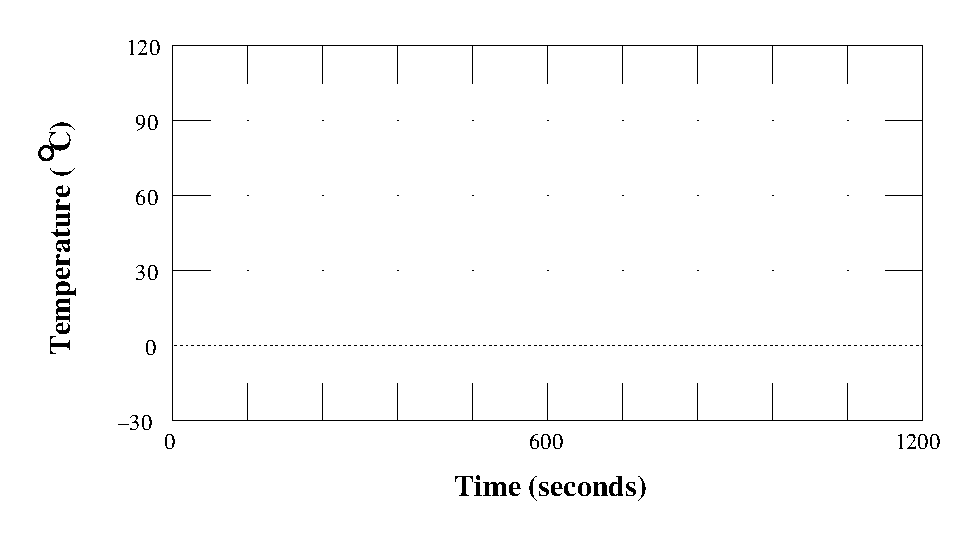
\includegraphics{heat/heat_temp_int_energy_fig_1.eps} \par}
\vspace{0.3cm}

\textbf{Activity \stepcounter{activity}\arabic{activity}: Measuring T vs. t for Water} 

(a) To test your prediction: 

\begin{enumerate}
\item Fill the glass beaker at least half full of ice water and set it on 
top of the hot plate.
\item Suspend the temperature probe so that the end is submerged in the ice 
water but not touching the side or bottom of the beaker. 
You will need to use the clamp and stand to do this.
\item Open the \textit{Heat, Temp, \& Internal Energy} application in the
132 Workshop folder on the {\bf Start} menu.
\item Turn on the hot plate and click the
\textbf{Start} button on the monitor to begin recording data. 
The temperature of the water will be recorded on the graph shown on the monitor. 
While there is still ice, stir gently. 
\item After the water begins to boil, turn off the hot plate and stop collecting 
data using the \textbf{Stop} button on the monitor. 
\item Sketch the shape of the measured heating curve on the above graph
using a solid line. Ignore small variations due to noise and uneven
heating. Mark the points at which the ice has melted and the water
begins to boil.
\end{enumerate}
(b) Does your prediction agree with the measured heating curve? If
not, what are the differences?
\vspace{20mm}

(c) What is the relationship between the temperature and the added
heat while the ice is melting?
\vspace{20mm}

(d) What is the relationship between the temperature and the added
heat after the ice has melted, but before the water begins to boil?
\vspace{20mm}

(e) What is the relationship between the temperature and the added
heat while the water is boiling?
\vspace{20mm}

(f) If there are regions of the heating curve in which the temperature
is not changing, what do you think is happening to the added heat
in these regions?\vspace{20mm}

%-------------------------------------------------------------------------



\setcounter{activity}{0}
\setcounter{equation}{0}
\setcounter{figure}{0}

\section{Calorimetry}

Name \rule{2.0in}{0.1pt}\hfill{}Section \rule{1.0in}{0.1pt}\hfill{}Date
\rule{1.0in}{0.1pt}

\textbf{Objective}

\begin{itemize}

\item To learn to use a method for measuring heat called calorimetry.

\item Measure the specific heat of aluminum and the heat of fusion of ice.

\end{itemize}

\textbf{Apparatus}

\begin{center}
\begin{tabular}{|l|l|l|} \hline
Hypsometer and stand & Hot plate            & Ice \\ \hline
Data Studio software & Temperature probe    & Clamp and stand \\ \hline
Safety goggles       & Aluminum pellets     & Compact scale           \\ \hline
Calorimeter          & Stirrers             &            \\ \hline
\end{tabular}
\end{center}

\textbf{Introduction to Calorimetry} 

Calorimetry is a method for measuring heat. As applied in this experiment,
the method involves the mixing together of substances initially at
two different temperatures. The substances at the higher temperature
lose heat and the substances at the lower temperature gain heat until
thermal equilibrium is reached.

\textbf{Activity \stepcounter{activity}\arabic{activity}: Statement of Conservation of Energy}

If no heat is transferred to the surroundings, what is the relationship
between the heat lost by the substances initially at high temperature
and the heat gained by the substances initially at low temperature?
Note: This is simply a statement of conservation of energy.

\vspace{0.3cm}
{\centering \resizebox*{!}{3.5in}{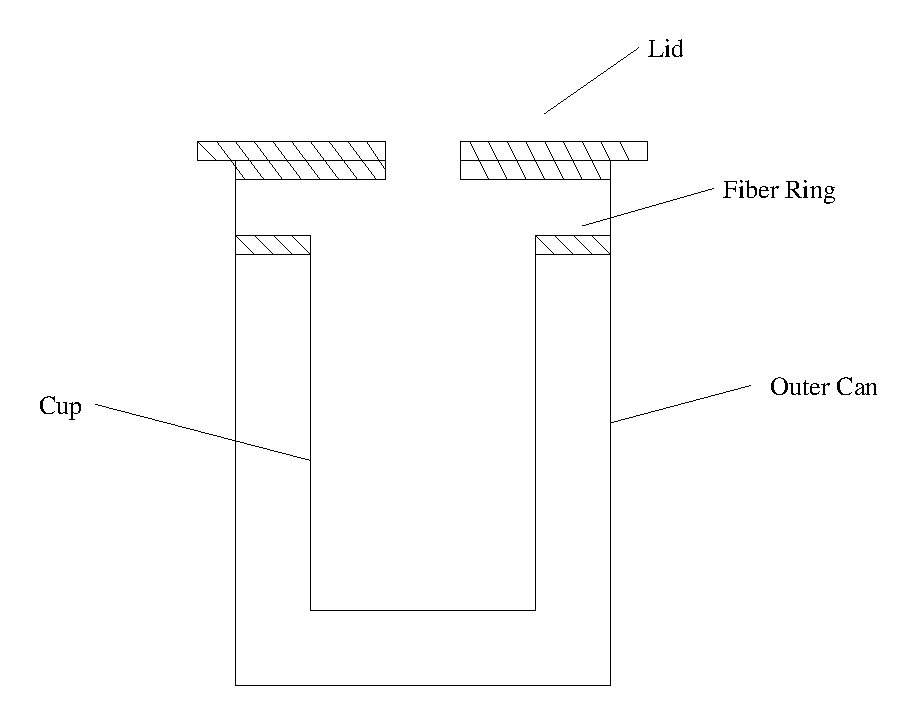
\includegraphics{heat/calorimetry_fig_1.eps}}  \par}
\vspace{0.3cm}

\textbf{Experimental Equipment} 

A calorimeter, shown in the above figure, is used in this experiment
to minimize the exchange of heat between the system and the surroundings.
The inner calorimeter cup is thermally insulated from the surroundings
by suspending it on a ring of material with low heat conductivity
and surrounding it with a layer of air. Also the cup is shiny to minimize
radiation loss. Hence, if the mixture of substances is placed inside
the calorimeter cup, the heat lost to or gained from the surroundings
can be ignored, and the above relationship can be used. The only part
of the calorimeter which is involved in the calculation is the inner
calorimeter cup which contains water and in which an exchange of heat
between the hot and cold bodies takes place. The cup will undergo
the same temperature change as the contained water. Of course, an
instrument will have to be introduced to measure the temperature of
the system, but the heat gained or lost by the instrument is small
and can be ignored.

\textbf{Activity \stepcounter{activity}\arabic{activity}: Specific Heat of Aluminum}

(a) Fill the hypsometer (boiler) at least half full of water and start
heating the water.

(b) Determine and record the mass of the hypsometer cup, m\( _{h} \).
Then fill it about half full with dry aluminum pellets. Determine
and record the mass of the cup and pellets, m\( _{hp} \), and calculate
the mass of the pellets, m\( _{p} \). Record the measurements in
the space below.
\vspace{15mm}

(c) Fill the plastic beaker with ice water. Open the \textit{Calorimetry}
application in the 132 Workshop folder in the {\bf Start} menu and start
collecting data. To make sure the temperature probe is working 
properly place it in the ice water and
check that it is reading approximately 0\( ^{\circ } \)C. If not,
then consult your instructor.

(d) Place the hypsometer cup in the top of the hypsometer and put the 
temperature probe into the middle of the pellets.  
To do this, remove the pellets from the cup, place the temperature probe in 
the proper position (using the clamp and stand), then return the pellets to the cup.

(e) Determine and record the mass of the calorimeter cup, m\( _{c} \).
Fill this cup about half full of cold tap water. Determine and record
the mass of the cup and water, m\( _{cw} \), and calculate the mass
of the water, m\( _{w} \). Then place the calorimeter cup in the outer
can and put the lid on.
\vspace{15mm}

(f) When the temperature of the pellets becomes constant, at or near
100\( ^{\circ } \)C, record the temperature of the pellets as T\( _{p} \).
Remove the probe from the pellets and put it in the cold water in the calorimeter cup. 
When the temperature of the water levels off, record it as T\( _{w} \).
\vspace{15mm}

(g) Now, quickly but carefully, pour the pellets into the water in
the calorimeter cup. Stir the water occasionally with the temperature probe and
monitor the temperature of the mixture. When the temperature levels off, record
this value as T. Click the {\bf Stop} button on the monitor, 
print your graph of temperature as a function of time and include it in this unit.
\vspace{15mm}

\newpage 

(h) Write the complete heat equation and solve for the unknown specific
heat of the metal. 
The specific heat of the calorimeter cup is 900 J/kg-\( ^{\circ } \)C.
\vspace{2in}

(i) Collect the other measurements of the specific heat from the other groups in
the class. 
Look up the accepted value for the specific heat of aluminum and
calculate the difference  between this value and the average.
Do the two values agree within experimental uncertainties?
Comment on possible sources of error.
\vspace{20mm}



\setcounter{activity}{0}
\section{Kinetic Theory of Ideal Gases\footnote{%
1990-93 Dept. of Physics and Astronomy, Dickinson College. Supported
by FIPSE (U.S. Dept. of Ed.) and NSF. Portions of this material may
have been modified locally and may not have been classroom tested
at Dickinson College.
}}

Name \rule{2.0in}{0.1pt}\hfill{}Section \rule{1.0in}{0.1pt}\hfill{}Date
\rule{1.0in}{0.1pt}

\textbf{Objective} 

\begin{itemize}
\item To derive a relationship between the macroscopic properties of an
ideal gas and the microscopic motion of the unseen atoms that make
up the gas. 
\end{itemize}

\textbf{Apparatus}

\begin{itemize}
\item A computer with an atomic and molecular motion simulation
\end{itemize}
\textbf{Introduction}

Do you believe in atoms? Our forefathers believed in the reality of
witches. In fact, they thought that they had good evidence that witches
existed, good enough evidence to accuse some people of being witches.
We believe in atoms. Are we truly more scientific than they were?

\textbf{Activity \stepcounter{activity}\arabic{activity}: Why Atoms!?}

(a) List reasons why you do or do not believe that matter consists
of atoms and molecules, even though you have never seen them with
your own eyes.
\vspace{20mm}

(b) What happens when heat energy is being transferred into a substance?
If you believe that substances are made of atoms and molecules, how
would you use their existence to explain the change in volume of a
heated gas?
\vspace{20mm}

\textbf{Models of Pressure Exerted by Molecules}

So far in physics we have talked about matter as if it were continuous.
We didn't need to invent aluminum atoms to understand how a ball rolled
down the track. But ever since the time of the fifth century B.C.
Greek philosophers Leucippus and Democritus, some thinkers have believed
in {}``atomism'', a picture of the universe in which everything
is made up of tiny {}``eternal'' and {}``incorruptible'' particles,
separated by {}``the void''. Today, we think of these particles
as atoms and molecules.

In terms of every day experience molecules and atoms are hypothetical
entities. In just the past 40 years or so, scientists have been able
to \char`\"{}see\char`\"{} molecules using electron microscopes and
field ion microscopes. But long before atoms and molecules could be
\char`\"{}seen\char`\"{} experimentally, nineteenth century scientists
such as James Clerk Maxwell and Ludwig Boltzmann in Europe and Josiah
Willard Gibbs in the United States used these imaginary microscopic
entities to construct models that made the description and prediction
of the macroscopic behavior of thermodynamic systems possible. Is
it possible to describe the behavior of an ideal gas that obeys the
first law of thermodynamics as a collection of moving molecules? To
answer this question, let's observe the pressure exerted by a hypothetical
molecule undergoing elastic collisions with the walls of a 3D box.
By using the laws of mechanics we can derive a mathematical expression
for the pressure exerted by the molecule as a function of the volume
of the box. If we then define temperature as being related to the
average kinetic energy of the molecules in an ideal gas, we can show
that kinetic theory is compatible with the ideal gas law and the first
law of thermodynamics. This compatibility doesn't prove that molecules
exist, but allows us to say that the molecular model would enable
us to explain the experimentally determined ideal gas law.

\textbf{Atomic Motion and Pressure}

Consider a spherical gas molecule that has velocity 
\( \overrightarrow{v}=v_{x} \)\( \hat{i}+v_{y} \)\( \hat{j} \)\( + v_z\hat k\) and
makes perfectly elastic collisions with the walls of a three-dimensional, cubical
box of length, width, and height $l$. Start the program called \char`\"{}\textit{Atoms
in Motion}\char`\"{} (in \char`\"{}\textit{Physics Applications}\char`\"{}). 
You will see a screen
like the one shown below. Experiment with it for a few moments. 
The {\it Run} and {\it Stop} buttons control the processing of the 
simulation of the gas atoms while the {\it Step} button allows you to watch the
`movie' one frame at a time.

\begin{figure}[hbt]
\begin{center}
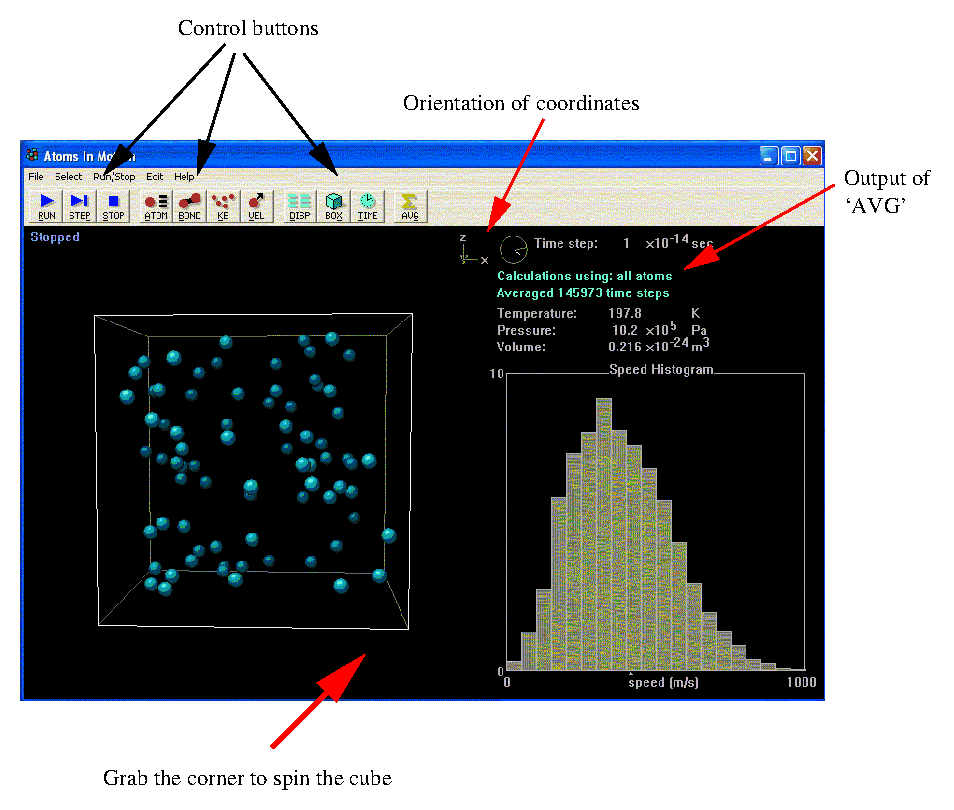
\includegraphics{kineticTheory/am4a.eps}
\caption{{\it Atoms in Motion} window.}
\end{center}
\end{figure}

Can we use the concept of molecules behaving like little billiard
balls to explain why the ideal gas law relationship might hold? In
the next activity you are to pretend you are looking under a giant
microscope at a single spherical molecule as it bounces around in
a three-dimensional box by means of elastic collisions and that you
can time its motion and measure the distances it moves as a function
of time. 

If the molecule obeys Newton's Laws, you can calculate how the average
pressure that the molecule exerts on the walls of its container is
related to the volume of the box. The questions we have to consider
are the following. What is the momentum change as the
molecule bounces off a wall? How does this relate to the change in
the velocity component perpendicular to the wall? How often will our
molecule \char`\"{}hit the wall\char`\"{} as a function of its component
of velocity perpendicular to the wall and the distance between opposite
walls? What happens when the molecule is more energetic and moves
even faster? Will the results of your calculations based on mechanics
be compatible with the ideal gas law?

\textbf{Activity \stepcounter{activity}\arabic{activity}: The Theory of Atomic Motion}

(a) Stop the simulation if it's running and set the number of molecules to 
one. Do this by clicking on the {\it ATOM} button and getting a dialog box.
Enter `1' for the
number of Type A atoms and zero for all the others. Record the mass of the
Type A atom. Click {\it OK} and
the cube should now contain a single atom. If not, consult your instructor.
\vspace{20mm}

(b) The orientation of coordinates can be seen just above the right-hand corner
of the cube (consult Figure 1 also).
Suppose the molecule moves a distance 2$l$ (across the cube and back) in the $x$-direction in
a time \( \Delta t_{x} \). What is the equation needed to calculate
its $x$-component of velocity in terms of $l$ and \( \Delta t_{x} \)?
\vspace{20mm}

(c) Suppose the molecule moves a distance 2$l$ in the $y$-direction in
a time \( \Delta t_{y} \). What is the equation needed to calculate
its $y$-component of velocity in terms of $l$ and \( \Delta t_{y} \)?
\vspace{20mm}

(d) Suppose the molecule moves a distance 2$l$ in the $z$-direction in
a time \( \Delta t_{z} \). What is the equation needed to calculate
its $z$-component of velocity in terms of $l$ and \( \Delta t_{z} \)?
\vspace{20mm}

(e) We will now measure the average time $\Delta t_y$ for one complete round trip
from the left side of the cube to the right side and back again.
Click {\it AVG} and you will see some information printed in the color blue
on the right-hand side of the {\it Atoms-in-Motion} window (see also Figure 1).
The simulation takes small steps in time and calculates the positions of the
atoms at the end of each time step.
The number of these time steps taken is shown on the right-hand side and the size 
of each time step is printed at the top, right-hand-side of the window.
Using the {\it Step} button let the atom in the cube move until it bounces off the 
left wall of the cube. 
Stop the motion and record the number of the time step in the space below.
\vspace{20mm}

\newpage

(f) Now run or step the simulation until the atom bounces across the cube, 
hits the right-hand wall, comes back and strikes the left hand wall again. 
Stop the motion and record the number of the time step.
Calculate $\Delta t_y$ and record it below.
\vspace{20mm}

(g) Each side of the cube has a length $l$ = $50 \times 10^{-10}$~m.
Combine this with the previous result to determine $v_y$ and record it.
\vspace{20mm}

(h) Repeat the above procedure for the top and bottom walls of the cube to get $v_z$.
\vspace{20mm}

(i) Rotate the cube by clicking and dragging one of the corners of the cube.
Spin it until you can see the atom bounces between the walls in the direction of
the $x$ coordinate.
Measure the $x$ component of the speed of the atom using the same procedure as before.
\vspace{20mm}

(j) Write the
expression for \( v_{total} \) in terms of the $x$, $y$, and $z$ components
of velocity. (Hint: This is an application of the 3-dimensional Pythagorean
theorem.) Determine $v_{total}$ for your atom.
We will use these results in a little while to calculate the pressure exerted by
our one-atom `gas'.
\vspace{20mm}

(k) Record the value of the pressure and temperature for your `gas' (as printed on the screen).
\vspace{20mm}

(l) We would like to eventually find the average kinetic energy of each atom or molecule
in a gas so we now have to think about a gas with many atoms.
Since the kinetic energy of a molecule is proportional to the square
of its total speed, you need to show that if \emph{on the average}
\( v_{x}^{2}=v_{y}^{2}=v_{z}^{2} \), then \( \overline{v_{total}^{2}}=3\overline{v_{x}^{2}} \).
\vspace{20mm}

\newpage

(m) If the collisions with the wall perpendicular to the $x$ direction
are elastic, show that the force exerted on that wall for each collision
is just \( F_{x}=2m\frac{v_{x}}{\Delta t_{x}} \)where m is the mass
of the particles and \( \Delta t_{x} \) the mean interval between
collisions with the wall. (Hint: Think of the form of Newton's second
law in which force is defined in terms of the change in momentum per
unit time so that \( F=\frac{\Delta p}{\Delta t} \).)

\textbf{Warning:} Physicists too often use the same symbol to stand
for more than one quantity. In this case, note that \( \Delta p \)
(where {}``p'' is in lower case) indicates the change in \emph{momentum},
not pressure.
\vspace{20mm}

(n) Substitute the expression from part (b) for \( \Delta t_{x} \)
to show that 

\[
F_{x}=\frac{mv_{x}^{2}}{l}\]

\vspace{20mm}

(o) We have assumed from the beginning that we have a cubical box of edge length $l$. Show
that the pressure on the wall perpendicular to the x axis caused by
the force \( F_{x} \) due to \emph{one} molecule is described by
the following expression.

\[
P=\frac{mv_{x}^{2}}{l^{3}}\]

\vspace{20mm}

(p) Let's say that there are not one but N molecules in the box. What
is the pressure on the wall now?
\vspace{20mm}

(q) Next, show that if we write the volume of our box as \( V=l^{3} \),
and recalling (part (l) above) that

\[
\overline{v_{x}^{2}}=\frac{\overline{v_{total}^{2}}}{3}\]


we can write the following expression.

\[
P=N\frac{m\overline{v_{total}^{2}}}{3V}\]

\vspace{20mm}

\newpage

(r) Finally, since the average kinetic energy of a molecule is just

\[
\overline{E_{kin}}=\frac{1}{2}m\overline{v_{total}^{2}}\]


show that the pressure in the box can be written in the following
way.

\[
P=\frac{2N\overline{E_{kin}}}{3V}\]
\vspace{20mm}

(s) Use the previous result to calculate the pressure using $v_{total}$, the mass of the
atom, $N$ and $V$ for your one-atom gas. Compare your result with the pressure 
you recorded above from the output of the simulation (part (k) above).
Do they agree? Explain any differences.
\vspace{20mm}


\setcounter{activity}{0}

\section{Applying the Kinetic Theory\footnote{%
1990-93 Dept. of Physics and Astronomy, Dickinson College. Supported
by FIPSE (U.S. Dept. of Ed.) and NSF. Portions of this material may
have been modified locally and may not have been classroom tested
at Dickinson College.
}}

Name \rule{2.0in}{0.1pt}\hfill{}Section \rule{1.0in}{0.1pt}\hfill{}Date
\rule{1.0in}{0.1pt}

\textbf{Objective}

\begin{itemize}
\item To derive the relationship between temperature and the kinematic properties
of the monatomic molecules of an ideal gas. We will also calculate
the specific heat per mole of an ideal, monatomic gas at constant
volume using the kinetic theory and compare the prediction with data.
\end{itemize}

\textbf{Apparatus}

\begin{itemize}
\item A computer with an atomic and molecular motion simulation
\end{itemize}

\textbf{Kinetic Energy, Internal Energy, and Temperature}

We have hypothesized the existence of non-interacting molecules to
provide the basis for a particle model of ideal gas behavior. We have
shown that the pressure of such a gas can be related to the average
kinetic energy of each molecule:

{\centering \( P=\frac{2N\left\langle E_{kin}\right\rangle }{3V} \)
or \( PV=\frac{2}{3}N\left\langle E_{kin}\right\rangle  \)\par}

Pressure increases with kinetic energy per molecule and decreases
with volume. This result makes intuitive sense. The more energetic
the motions of the molecules, the more pressure we would expect them
to exert on the walls. Increasing the volume of the box decreases
the frequency of collisions with the walls, since the molecules will
have to travel longer before reaching them, so increasing volume should
decrease pressure if \( \left\langle E_{kin}\right\rangle  \) stays
the same.

\textbf{The Molar Specific Heat}

The kinetic theory of gases uses the atomic theory to relate the macroscopic
properties of gases to the microscopic features of the atoms and molecules
that make up the gas. In this laboratory we will extend the calculations
that we have made so far to include the molar specific heat of an
ideal, monatomic gas. The success of that extension of the theory
depends on how well the calculations reproduce the measured heat capacities
of a variety of real (not ideal) gases.

\textbf{Activity \stepcounter{activity}\arabic{activity}: Experimenting with the Gas Simulation Program}

Open the {\it Atoms in Motion} program (in {\it Physics Applications}) on the {\it Start} menu.
We are first going to explore the relationship between pressure and volume in
our kinetic theory using the simulation. 

(a) According to the ideal gas law \( PV = nRT = Nk_{B}T \), where \( R \) is the 
universal gas constant and \( k_{B} \) is Boltzmann's constant. What
should happen to the pressure of an ideal gas as its volume increases
or decreases?
\vspace{1.0in}

(b) We now want to run a more realistic simulation.
Under the {\it ATOM} menu set the number of Type A atoms to 50 and set all the others to zero.
Click on the {\it BOX} button and a new dialog box will appear.
Check the box beside `Floor conducts heat' and set the temperature to $200~K$.
Notice at the top that the box width is $l=50 \times 10^{-10}~m$.
We have now set up a situation where one side of the cube is held at a constant
temperature ({\it e.g.} it's sitting on a stove) so the collisions of the atoms with the
floor are no longer elastic.
The remaining sides of the
cube do not transfer any energy (they're insulated) so elastic collisions still occur 
at those walls.

Start
the simulation and make sure you are averaging the pressure over many time steps.
You should see the number of averaged time steps increasing on the right-hand side 
of the {\it Atoms-in-Motion} window. 
If you don't see this information, click on {\it AVG} and it should appear.

(c) What happens to the pressure?
What happens to the temperature of the gas? 
You will find that it can take several minutes of computer time for the temperature 
of the gas to reach equilibrium with the floor.
Once the gas temperature is within $8-10~K$ of the floor temperature, 
we can consider the gas and the floor to be in thermal equilibrium. 
Record the volume, pressure and temperature of the gas in the first line of the table below.
\vspace{20mm}

(d) Record the volume, pressure and temperature of the gas for five more volumes of the cube. Change the volume of the cube using the
{\it BOX} menu and adjusting the box width. The volume is printed on the
{\it Atoms-in-Motion} window.
Plot your results and attach the graph
to this unit. Are your results consistent with the ideal gas law and
your prediction in part (a)? Are they consistent with the results of Experiment 4?
%\vspace{1.5in}

\vspace{0.3cm}
{\centering \begin{tabular}{|c|c|c|}
\hline 
~~~~{}Volume of Box~~~~&
~~~~Average Pressure~~~&
~~~~~~Temperature~~~~~~~\\
\hline
\hline 
& &
\\
\hline 
& &
\\
\hline 
& &
\\
\hline 
& &
\\
\hline 
& &
\\
\hline 
& &
\\
\hline
\end{tabular}\par}
\vspace{0.3cm}

(e) In the procedure above you should have found the pressure to be inversely
proportional to the volume. How could you modify your plot to show
the pressure is proportional to \( 1/V \)? Make such a plot and fit it.
How close is your data to following a straight line? Attach the plot
to this unit.
\vspace{1.5in}

(f) According to the ideal gas law \( PV = nRT = Nk_{B}T \). What
should happen to the pressure of an ideal gas as the number of particles
increases or decreases?
We will explore this idea with the simulation next.
\vspace{1.5in}

(g) Start off with the gas parameters from the last `run' of the 
simulation.
Record the number of atoms, temperature, and pressure in the table below.
Use the {\it ATOM} menu to change the number of atoms (or molecules) in the cube.
Start
the simulation. What happens to the pressure? Record the pressure
and the number of molecules for four more values of the number of
molecules and plot your results. Attach the plot to this unit. Are your results consistent with
the ideal gas law and your prediction in part (f)?
\vspace{1.5in}

\vspace{0.3cm}
{\centering \begin{tabular}{|c|c|c|}
\hline 
~~~~Number of Molecules~~~~&
~~~~Average Pressure~~~~&
~~~~~~Temperature~~~~~~~\\
\hline
\hline 
& &
\\
\hline 
& &
\\
\hline 
& &
\\
\hline 
& &
\\
\hline 
& &
\\
\hline
\end{tabular}\par}
\vspace{0.3cm}

\textbf{Kinetic Theory and the Definition of Temperature}

The model of an ideal gas we have just derived requires that

{\centering \( PV=\frac{2}{3}N\left\langle E_{kin}\right\rangle  \)\par}

But we have determined experimentally the ideal gas law:

{\centering \( PV = Nk_{B}T \)\par}

What can we say about the average kinetic energy per molecule for
an ideal gas? You can derive a relationship between temperature and
the energy of molecules that serves as a microscopic (i.e. molecular)
definition of temperature.

\textbf{Activity \stepcounter{activity}\arabic{activity}: Microscopic Definition of Temperature}

(a) From the two equations above, derive an expression relating \( \left\langle E_{kin}\right\rangle  \)
and \( T \). Show the steps in your derivation.
\vspace{1.5in}

\newpage

(b) In general, molecules can store energy by rotating or vibrating,
but for an ideal gas of \emph{point} particles (monatomic gas), 
the only possible form of kinetic energy is the translational motion of the particles. 
If we can ignore potential energy due to gravity or electrical forces, then the internal
energy \( E_{int} \) of a gas of \( N \) particles is \( E_{int}=N\left\langle E_{kin}\right\rangle  \).
Use this to show that for an ideal gas of point particles, E\( _{int} \)
\emph{depends only on N and T}. Derive the equation that relates \( E_{int} \),
\( N \) and \( T \). Show the steps.
\vspace{1.5in}

The microscopic and the macroscopic definitions of temperature are
equivalent. The microscopic definition of temperature which you just
derived is fundamental to the understanding of all thermodynamics!

\textbf{Activity \stepcounter{activity}\arabic{activity}: Calculating the Molar Specific Heat}

In this section we will generate a series of equations that we will
then bring together in order to predict the molar specific heat at
constant volume.
\vspace{1in}

(a) Consider an ideal gas in a rigid container that has a fixed volume.
How is the molar specific heat defined in terms of the heat added \( Q \)?
\vspace{1in}

(b) If the gas is heated by an amount \( Q \), then how much work is done
against the fixed container? Recall the first law of thermodynamics
and incorporate this result into your statement of the first law.
\vspace{1in}

(c) Now use the equations of parts (a) and (b) to relate the change
in internal energy \( \Delta E_{int} \) to the molar specific heat.
\vspace{1in}

%(d) We now want to find another expression for the change in internal
%energy \( \Delta E_{int} \) that is related to the average kinetic
%energy of the particles in the gas. How do you think the internal
%energy of an ideal, monatomic gas is related to \( \left\langle E_{kin}\right\rangle  \)
%(notice you are calculating the internal energy \( E_{int} \) here,
%not \( \Delta E_{int} \))?
%\vspace{1in}

\newpage

(d) Write down an expression for  the change in internal
energy of the ideal gas in terms of \( \left\langle E_{kin}\right\rangle  \).
(Suggestion: see part (b) of Activity 2.)
How is \( \left\langle E_{kin}\right\rangle  \) related to the temperature?
Incorporate this relationship into your expression for the change
in the internal energy. You should find that

{\centering \( \Delta E_{int}=\frac{3}{2}Nk_{B}\Delta T \)\par}

where \( k_{B} \) is Boltzmann's constant and N is the number of
molecules in the gas.
\vspace{1in}

(e) Use the equations is parts (c) and (d) to relate the molar specific
heat to the number of particles \( N \) and Boltzmann's constant \( k_{B} \).
You should find that
\vspace{1in}

{\centering \( nC_{V}=\frac{3}{2}Nk_{B} \)\par}

where \( n \) is the number of moles.
\vspace{1.5in}

(f) How is the number of molecules in the gas \( N \) related to the number
of moles \( n \) and Avogadro's number \( N_{A} \)? Use this expression
and the result of part (e) to show

{\centering \( C_{V}=\frac{3}{2}N_{A}k_{B} \) or \( \frac{C_{V}}{N_{A}k_{B}}=\frac{3}{2} \)\par}
\vspace{1.5in}

Since \( N_{A}k_{B}=R \), this can be written as

{\centering \( C_{V}=\frac{3}{2}R \) or \( \frac{C_{V}}{R}=\frac{3}{2} \)\par}
\vspace{0.3in}

\newpage

\textbf{Activity \stepcounter{activity}\arabic{activity}: Comparing Calculations and Data}

We now want to compare our calculation of the molar specific heat
of an ideal, monatomic gas with the measured molar specific heats
of some real gases. The table below lists some of those measurements.

\vspace{0.3cm}
{\centering \begin{tabular}{|c|c|c|c|}
\hline 
Molecule&
\( \frac{C_{V}}{R} \)&
Molecule&
\( \frac{C_{V}}{R} \)\\
\hline
\hline 
He&
1.50&
CO&
2.52\\
\hline 
Ar&
1.50&
Cl\( _{2} \)&
3.08\\
\hline 
Ne&
1.51&
H\( _{2} \)O&
3.25\\
\hline 
Kr&
1.49&
SO\( _{2} \)&
3.77\\
\hline 
H\( _{2} \)&
2.48&
CO\( _{2} \)&
3.42\\
\hline 
N\( _{2} \)&
2.51&
CH\( _{4} \)&
3.25\\
\hline 
O\( _{2} \)&
2.53&
&
\\
\hline
\end{tabular}\par}
\vspace{0.3cm}

(a) Has our theoretical calculation been successful at all? Which
gases appear to be consistent with our calculation? Which gases are
not? How do these two groups of real gases differ?
\vspace{1in}

(b) Can you suggest an explanation for the partial success of the
theory? Which one of the original assumptions that went into our kinetic
theory might be wrong?\vspace{2in}



\setcounter{activity}{0}
P7 332
#XVVERSION:version 3.10a-jumboFix+Enh of 20081216 (interim!)+FLmask
#BUILTIN:UNKNOWN
#IMGINFO:
#END_OF_COMMENTS


% appendices.

P7 332
#XVVERSION:version 3.10a-jumboFix+Enh of 20081216 (interim!)+FLmask
#BUILTIN:UNKNOWN
#IMGINFO:
#END_OF_COMMENTS


P7 332
#XVVERSION:version 3.10a-jumboFix+Enh of 20081216 (interim!)+FLmask
#BUILTIN:UNKNOWN
#IMGINFO:
#END_OF_COMMENTS


P7 332
#XVVERSION:version 3.10a-jumboFix+Enh of 20081216 (interim!)+FLmask
#BUILTIN:UNKNOWN
#IMGINFO:
#END_OF_COMMENTS



\section{Video Analysis}

\textbf{Making a Movie with ``Windows Live Movie Maker''} 

To make a movie, perform the following steps:

\begin{enumerate}

\item Make sure the camera is connected to a USB port on your computer. 
Close all windows, applications, programs, and browsers.

\item Click the {\bf Start} button in the lower-left corner of your screen and type `movie maker' in the Search programs and files box. 
Once the search results appear, click on {\bf Windows Live Movie Maker} under {\bf Programs}. 
After movie maker starts, close any pop-up windows that may appear.

\item Click the {\bf Webcam Video} button. 
A webcam video window opens. 
Enlarge the video frame by dragging the vertical line on the right side of the video frame.

\item Position the camera 2-3 meters from the object you will be viewing. 
Adjust the camera height and orientation so that the field of view is 
centered on the expected region where the object will move. 

\item Place a meter stick or an object of known size in the field of view where 
it won't interfere with the experiment. 
The meter stick should be the same distance away from the camera as the motion 
you are analyzing so the horizontal and vertical scales will be accurately determined. 
It should also be parallel to one of the sides of the movie frame. 
Make sure that the meter stick is not far away from the central region of field of view, and that it is perpendicular to the line of sight of camera.

\item One member of your group should perform the computer tasks while the other does the experiment.

\item To start recording your video, click {\bf Record}. When you are done, click {\bf Stop}. 

Save the video on your Desktop with a unique name that you can easily identify.
 The video will be saved in Windows Media Video format, i.e. with extension wmv. (Do not save the video as a Movie Maker Project file.)

\end{enumerate}

\textbf{Analyzing the Movie} 

To determine the position of an object at different times during the
motion, perform the following steps:

\begin{enumerate}

\item Start up Tracker by going to {\bf Start} $\rightarrow$ {\bf All Programs} $\rightarrow$ 
{\bf Physics Applications} $\rightarrow$ {\bf Tracker}. 
When {\bf Tracker} starts it appears as shown below. The menu icons and buttons that we will use are identified by arrows.
\begin{figure}[hbt]
\begin{center}
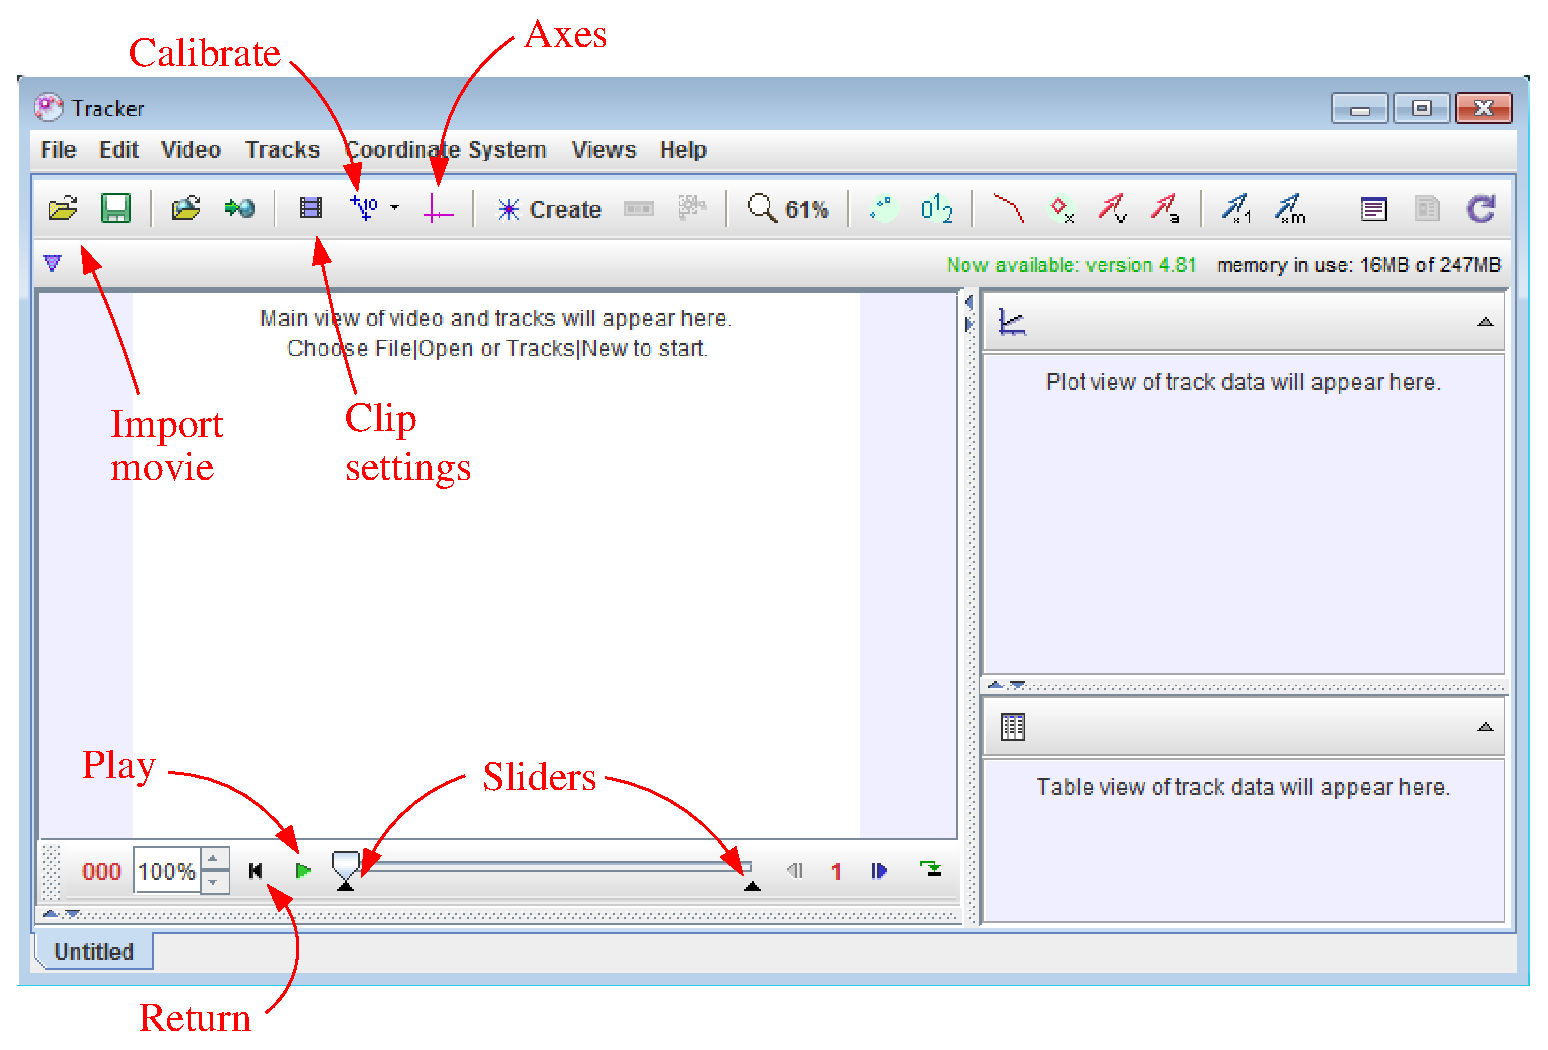
\includegraphics[width=5.5in]{appendices/video_analysis_tracker_fig1d.eps}
\caption{Initial {\bf Tracker} window for video analysis.}
\end{center}
\end{figure}

\item Click the {\bf Open Video} button on the toolbar (see figure below) to import your video. 
After your video is imported, Tracker will warn you that the video frames don't have the same time duration. 
This is okay since Windows Live Movie Maker uses a variable frame rate. 
Click {\bf Close} on the warning window to ignore Tracker's recommendation.

\item Click the {\bf Clip Settings} button (see figure below) to identify the frames you wish to analyze. 
A clip settings dialog box appears. 
Here, you only need to identify and set the start and end frames. 
Leave everything else in the dialog box unchanged. 
To find and set the start frame, drag the player's left slider to scan forward through the video, and 
stop when you get to the first frame of interest. 
Now, the start frame is set and the corresponding frame number should be displayed in the dialog box. 
If not, then click on the {\bf Start Frame} in the dialog box, enter the number of the frame 
(printed in the lower right part of the Tracker window), and click outside the box.
Then, click the {\bf Play video} button to go to the last frame in the video. 
Next, drag the player's right slider to scan backward through the video to find the last frame of interest. 
Stop when you get to the frame of interest. Now, the end frame is also set and the corresponding frame number should be displayed in the dialog box. 
If not, then click on the {\bf End Frame} in the dialog box, enter the number of the frame, and click outside the box.
Finally, click the {\bf OK} button to close the dialog box, and then click the player's {\bf Return} button to return to the start frame.

\item Click the {\bf Calibration} button (see the figure) and select the {\bf calibration stick}. 
A blue calibration line appears on the video frame. 
Drag the ends of this blue line to the ends of your calibration meter stick. 
Then click the readout box on the calibration line to select it. 
Enter the length of the meter stick in this box (without units). 
For example, if your calibration meter stick is 1.00 meter long, enter 1.00 in the box 
and then click outside the box to accept the value or hit {\bf Return}. 
At this point, you can right-click the video frame to zoom in for more accurate adjustment of the ends 
of the calibration stick. 
Right-click the video again to zoom out.

\item Click the {\bf Axes} button (see the figure) to set the origin and orientation of the x-y coordinate axes. 
Drag the origin of the axes to the desired position (in most cases the initial position of the object of interest). 
Click the video outside the origin to fix the position of the origin. 
To change the orientation (angle) of the axes, drag the x axis. 
Click the video to fix the new orientation.

\item Click the {\bf Create} button (see the figure) to track the object of interest in the video. 
From the menu of choices select {\bf Point Mass} for the track type. 
Make sure the video is at the start frame, which shows the initial position of the object of interest. 
Mark this position by holding down the {\bf shift key} and clicking the mouse (crosshair cursor) on the object. 
As the position is marked, the video automatically advances to the next frame. 
Similarly, mark the position of the object on this and subsequent frames by holding down the {\bf shift key} 
and clicking the mouse. 
Do not skip any frames. 

After marking the position on the end frame, you can adjust any one of the marked positions. 
Advance the video to the frame where you would like to make a fine adjustment. 
Right-click the video frame to zoom in and drag the marked position with the mouse.

If you would like to track additional objects, repeat the procedure outlined here for each object.

\item Click the {\bf Set track length} button (see the figure) to get a drop-down menu that
will enable you to show all of the points you marked on the frame.

\item {\bf Plotting and Analyzing the Tracks:} The track data (position versus time) are listed in the Table View 
and plotted in Plot View sections of the Tracker screen. 
Click the vertical axis label of the plot to change the variable plotted along that axis. 
To plot multiple graphs, click the {\bf Plot} button, located above the plot, and select the desired number. 

Right-click on a plot to access display and analysis options in a pop-up menu. 
To fit your data to a line, parabola, or other functions, select the {\bf Analyze} option. 
On the Data-Tool window that opens up, click on the {\bf Analyze} tab at the top of the plot and 
check the {\bf Curve Fits} box. Select the fit type from the {\bf Fit Name} drop-down menu.
Make sure the {\bf Auto Fit} box is checked.


Note that the curve fitter fits the selected function to the data in the two leftmost columns of the displayed data table. 
The leftmost column, identified by a yellow header cell, defines the independent variable, and the second leftmost column, 
identified by a green header cell, defines the dependent variable. 
So, to fit the data in other columns, their corresponding headers must be dragged to the two leftmost columns.


\item {\bf Printing and Exporting Data:} Track data can also be easily exported to Excel for 
further analysis by copying the data from the 
data table to the clipboard and pasting into Excel. 
Click the {\bf Table} button, located above the data table in the table view section of the main screen, 
and select from the displayed list the data you would like to display in the data table. 
Select the desired data in the table by clicking and dragging, then right-click and choose {\bf Copy Data} 
from the pop-up menu. 
Now, paste the data into Excel.
To print out the displayed  plot or data table on Tracker's screen, 
right-click on the plot or table and choose Print from the pop-up menu.

\end{enumerate}



P7 332
#XVVERSION:version 3.10a-jumboFix+Enh of 20081216 (interim!)+FLmask
#BUILTIN:UNKNOWN
#IMGINFO:
#END_OF_COMMENTS


\end{document}
